\section{Examples of methods}\label{sec:examples-methods}
This section will present examples of how the linear and nonlinear methods behave on linear and nonlinear data. It should be noted again that the methods have different purposes. As a quick reminder, \gls{pca} tries to maximize the variance in the embedded data (and so does \gls{kpca}). In contrast, \gls{lda} tries to maximize the separability of classes in the data, and \gls{isomap} tries to preserve the distances from the high-dimensional data when projecting it onto a lower space. Therefore their results will not be a one-to-one comparison. All of the methods used in this section are implemented from Scikit-learn~\cite{scikit-learn}.

\subsection{Linear data example}\label{subsec:linear-data-example}
As linear data, we will use the Iris dataset, which contains three different species of Iris flowers, with 50 examples each. Each class has four dimensions: the length and width of the sepals and petals~\cite{iris-dataset}. The dataset is a simple and well-known dataset, which has been used in many machine learning papers~\cite{iris-dataset} and should give intuition as to how the methods behave on the dataset.

\begin{figure}[htb!]
    \centering
    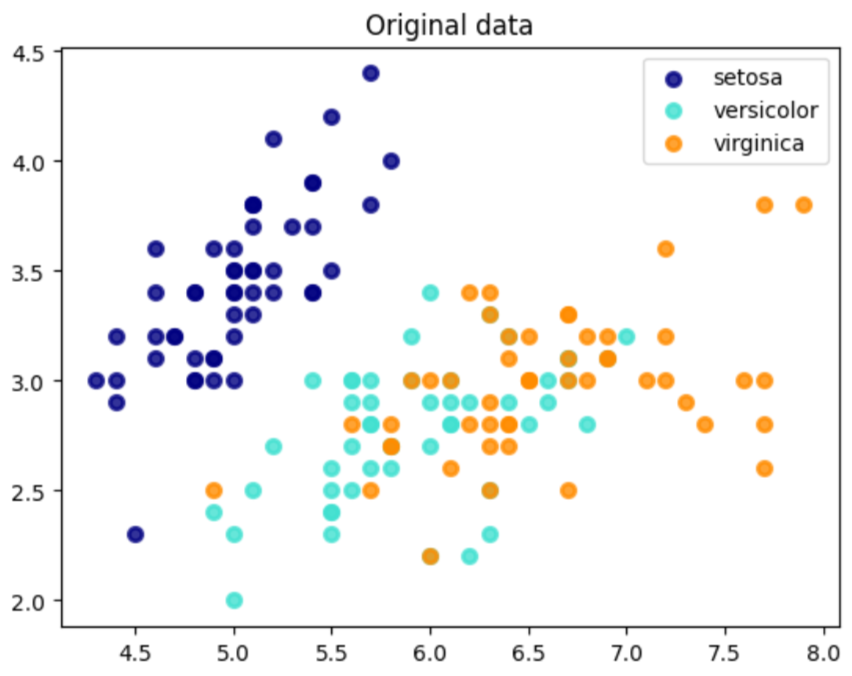
\includegraphics[width=0.5\textwidth]{figures/theory-example-figures/linear-data.png}
    \caption{Linear data as Iris dataset}
    \label{fig:linear-data}
\end{figure}

Figure \ref{fig:linear-data} represents the iris flowers on a 2D plot. According to~\cite{iris-dataset}, only one class is separable, which can further be solidified by the fact that the species Setosa is the only visually linearly separable class. 

\subsubsection{Linear methods}\label{subsubsec:linear-methods-on-iris}
In figure \ref{fig:iris-pca}, one can see that \gls{pca} has successfully separated the Setosa species from Versicolor and Virginica in the dataset. The other species are not separated on the coordinates [1.20, -0.20]. Having only Setosa separated from Versicolor and Virginica in the dataset is not concerning, as the test on the Iris dataset is to separate Setosa from the other classes by linear separability.

\begin{figure}
    \centering
    \subfloat[\centering LDA on iris]{\label{fig:iris-lda}{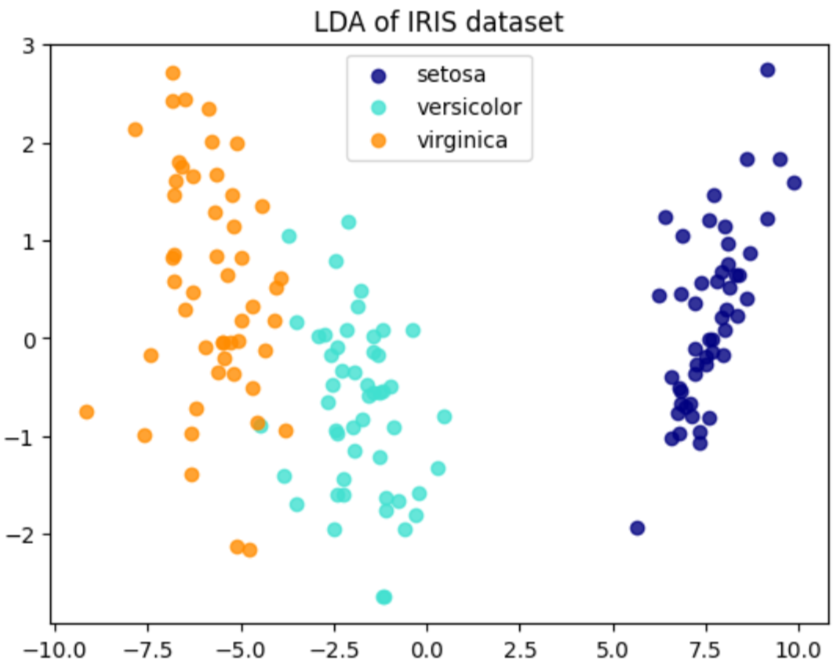
\includegraphics[width=0.4\textwidth]{figures/theory-example-figures/iris-lda.png} }}
    \qquad
    \subfloat[\centering PCA on iris]{\label{fig:iris-pca}{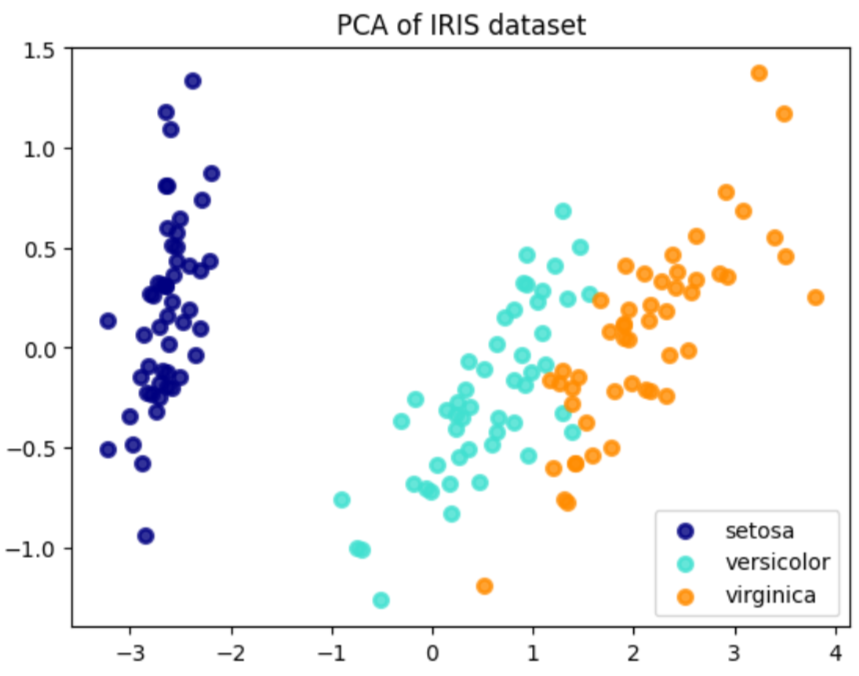
\includegraphics[width=0.4\textwidth]{figures/theory-example-figures/iris-pca.png} }}%
    \caption{both linear methods on iris}
    \label{fig:linear-methods-iris}
\end{figure}

In Figure \ref{fig:iris-lda}, \gls{lda} has also successfully separated the Setosa species from the other classes in the dataset. In contrast with \gls{pca}, \gls{lda} has managed to separate somewhat better as the distinction between those classes can be made more accessible. An advantage that \gls{lda} poses is that \gls{lda} is a supervised method, which means that  \gls{lda} knows the labels of the data and may be better suited for classifying the data.


\subsubsection{Nonlinear methods}\label{subsubsec:nonlinear-methods-on-iris}
In Figure \ref{fig:iris-isomap}, \gls{isomap} has tried to separate the Setosa and map the data on the first two dimensions. \gls{isomap}, as opposed to the aforementioned linear methods, has found little diversity on the second projection, as the values range from approximative 0.0 to -0.25. Such a range is short in comparison with the linear methods. \gls{isomap} clusters the Setosa species, but that may not be helpful if the data needs to be projected on two dimensions. If, for example, a point is in the upper left corner, it is impossible to tell if it is a Setosa or a Versicolor. \gls{isomap} is nevertheless a nonlinear method, and it is expected that it does not reduce the data as efficiently as the linear methods.

\begin{figure}
    \centering
    \subfloat[\centering Isomap on iris]{\label{fig:iris-isomap}{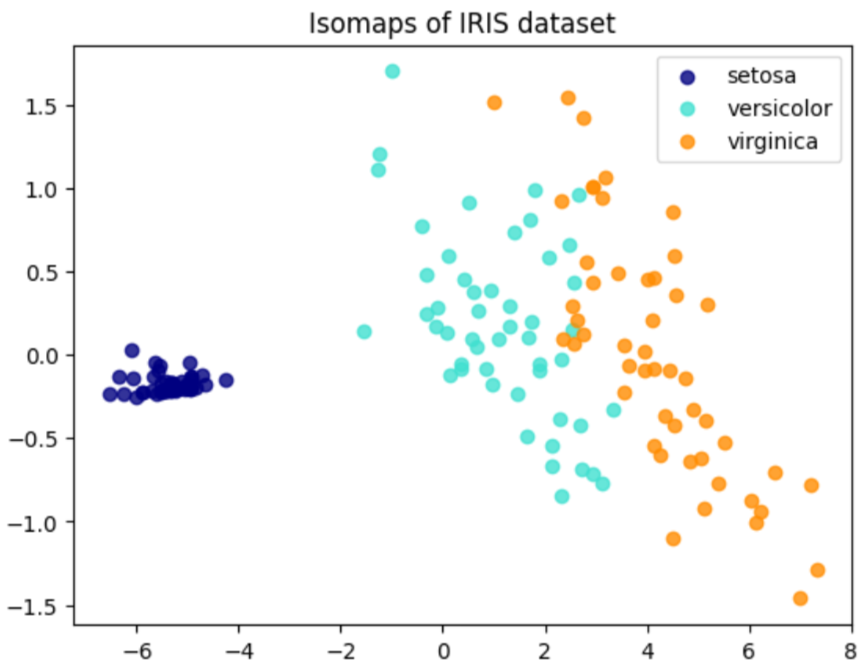
\includegraphics[width=0.4\textwidth]{figures/theory-example-figures/iris-isomap.png} }}
    \qquad
    \subfloat[\centering KernelPCA on iris]{\label{fig:iris-kernelpca}{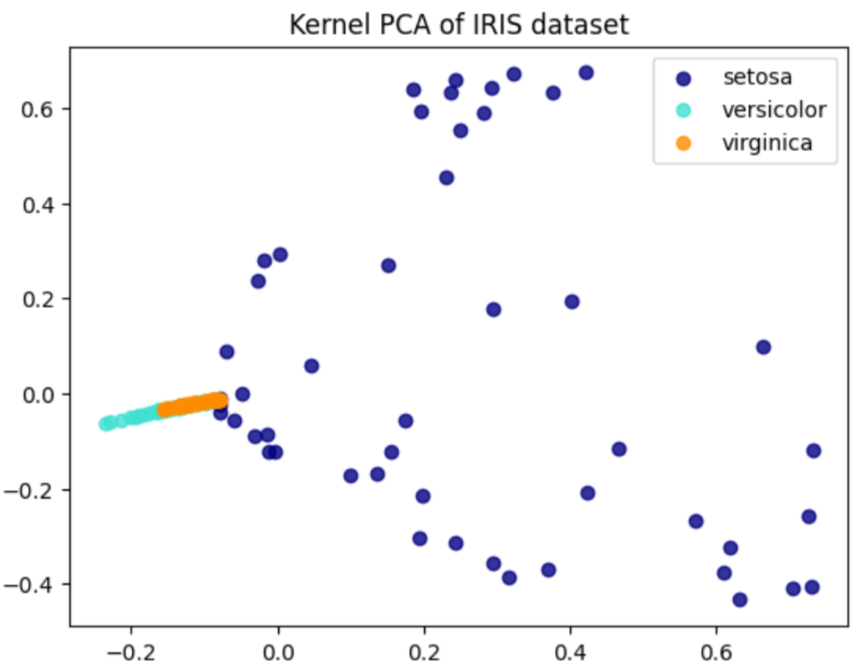
\includegraphics[width=0.4\textwidth]{figures/theory-example-figures/iris-kernelpca.png} }}
    \caption{both nonlinear methods on iris}
    \label{fig:nonlinear-methods-iris}
\end{figure}

In figure \ref{fig:iris-kernelpca}, \gls{kpca} has tried to separate the Setosa. In the figure, it can be seen that \gls{kpca} has clustered the other two species on the first projection, but there cannot be any clear separation between them, especially on the second projection. \gls{kpca} has also mapped the data points for Setosa with a high degree of variance, but it did not separate the Setosa from the other two species. Likewise, \gls{isomap} and \gls{kpca} were not supposed to separate the data and the linear methods. However, it is interesting that \gls{kpca} has yet to separate the Setosa species from the rest of the data.


\subsection{Nonlinear data example}\label{subsec:nonlinear-data-example}
As nonlinear data, we will construct two classes of circles, an inner- and an outer circle, which will look like in Figure \ref{fig:circles}.

\begin{figure}[htb!]
    \centering
    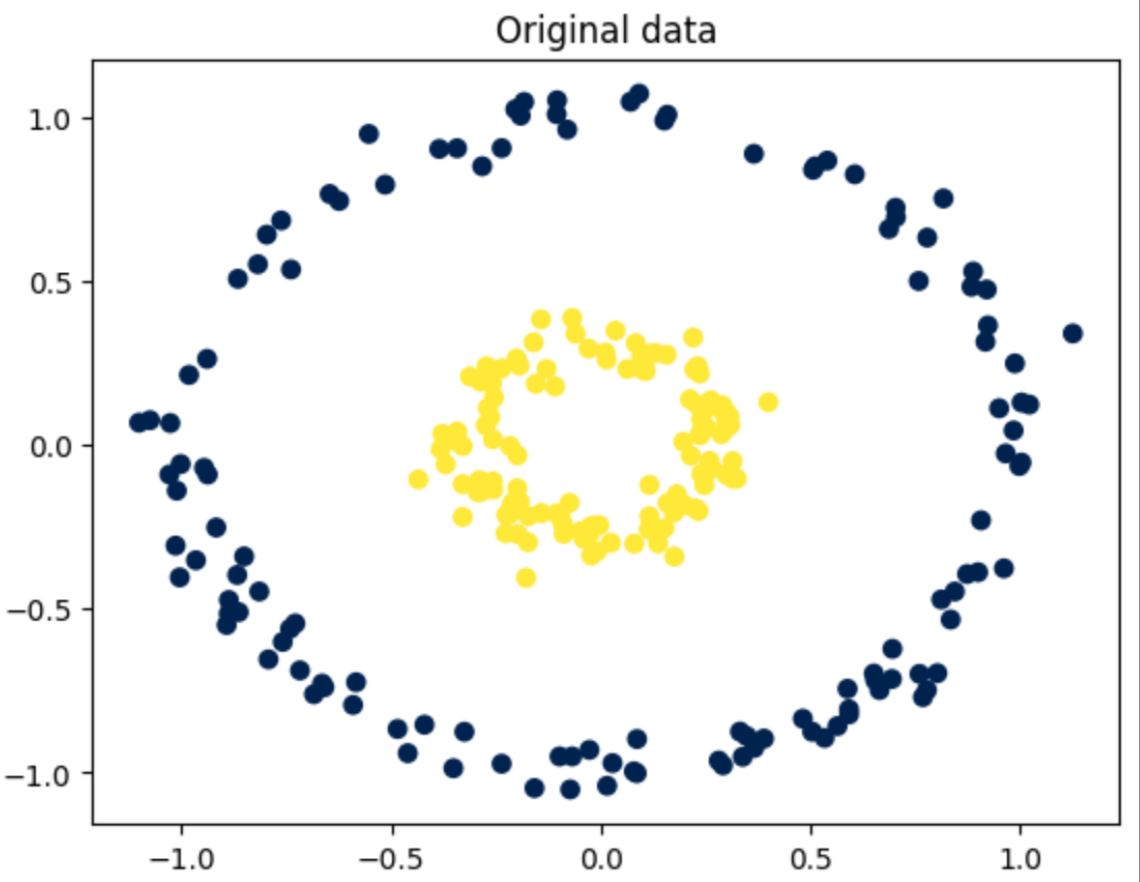
\includegraphics[width=0.5\textwidth]{figures/theory-example-figures/fig-circles.png}
    \caption{Nonlinear data as two circles}
    \label{fig:circles}
\end{figure}

\subsubsection{Linear methods}\label{subsubsec:linear-methods-on-circles}
In Figure \ref{fig:circles-pca}, it can be seen that \gls{pca}'s transformation could have managed to map the nonlinear data. In Figure \ref{fig:circles-lda}, \gls{lda} has reduced the data's dimensions to one dimension, but the two classes are clustered, which means that \gls{lda} could not separate the two classes.

\begin{figure}
    \centering
    \subfloat[\centering LDA on circles]{\label{fig:circles-lda}{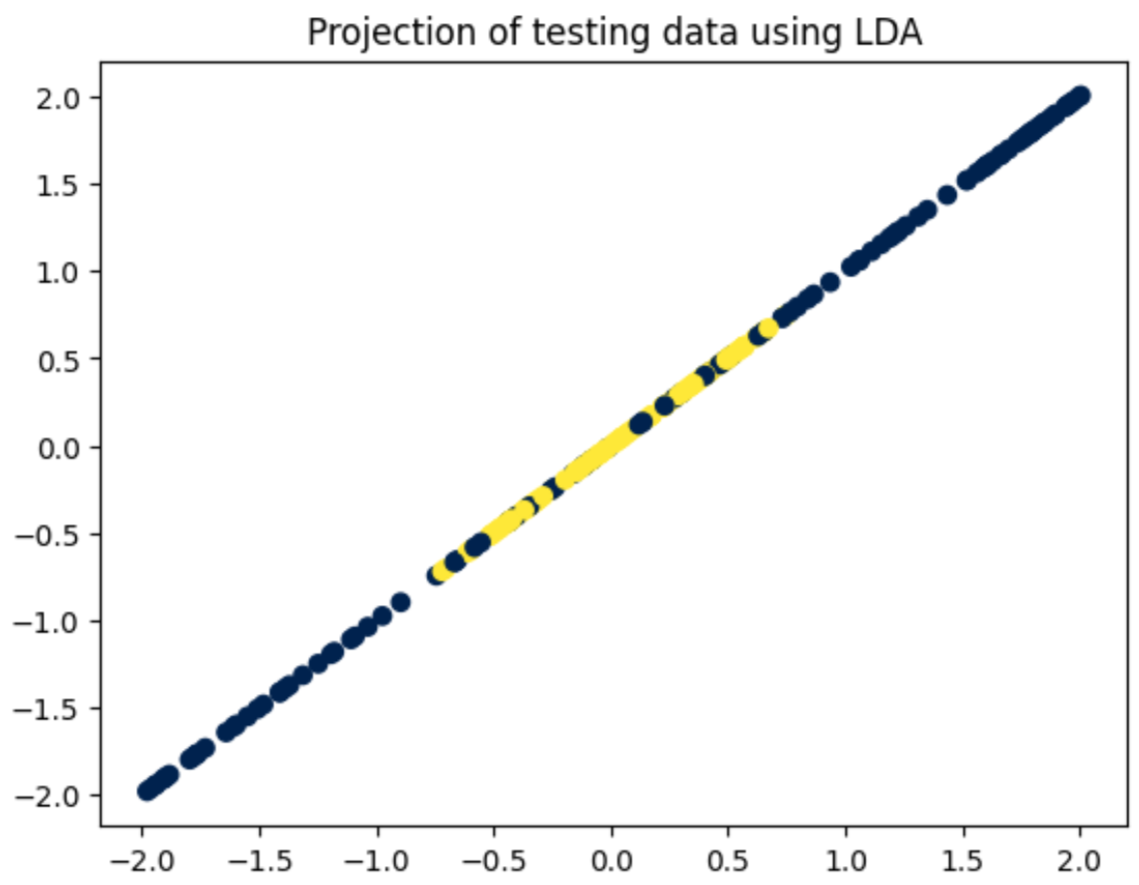
\includegraphics[width=0.4\textwidth]{figures/theory-example-figures/circles-lda.png} }}
    \qquad
    \subfloat[\centering PCA on circles]{\label{fig:circles-pca}{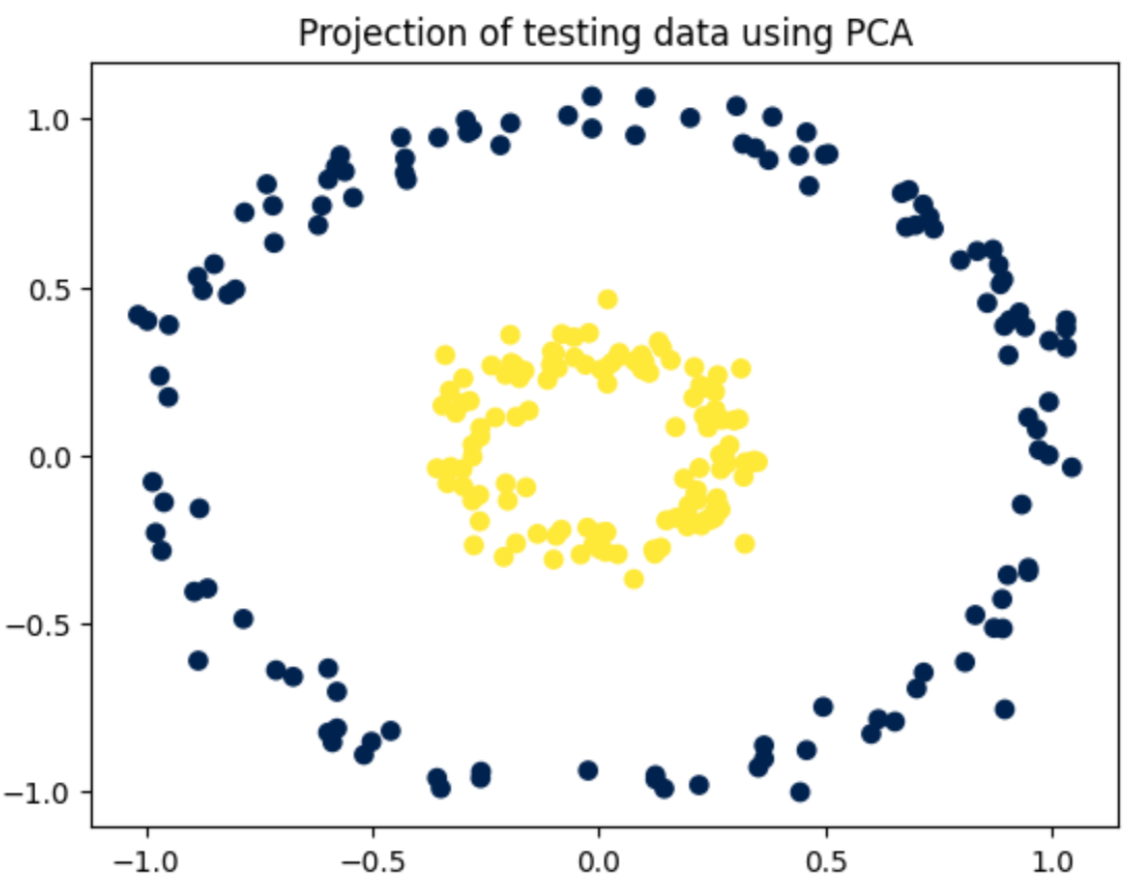
\includegraphics[width=0.4\textwidth]{figures/theory-example-figures/circles-pca.png} }}
    \caption{both linear methods on circles}
    \label{fig:linear-methods-circles}
\end{figure}

\subsubsection{Nonlinear methods}\label{subsubsec:nonlinear-methods-on-circles}
In Figure \ref{fig:circles-isomap}, \gls{isomap} has separated the data points from the circles. Based on the first projection \gls{isomap} is capable of separating the data. On the second projection, the method can capture more information about the outer circle, thus approximating the original data. The outer circle has a higher variance than the inner circle. The second projection, \gls{isomap}, revealed little information about the inner circle.

\begin{figure}
    \centering
    \subfloat[\centering Isomap on circles]{\label{fig:circles-isomap}{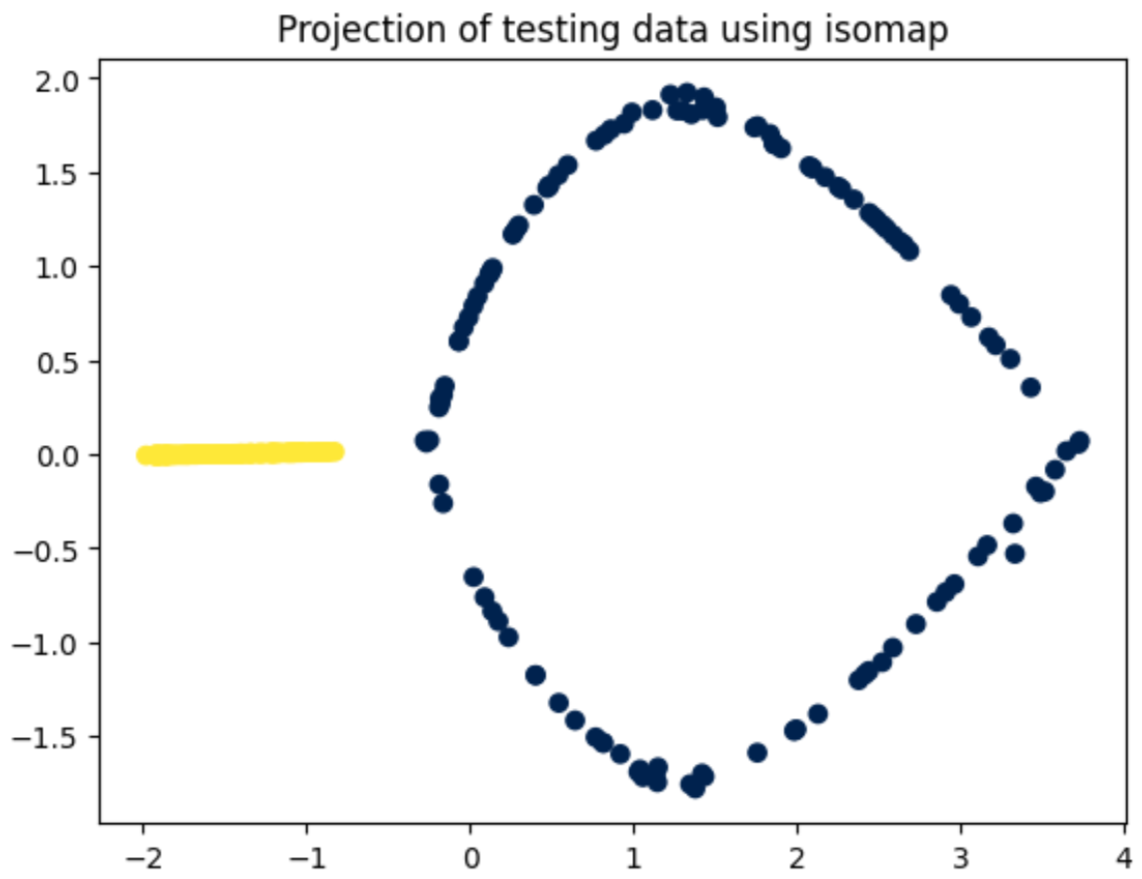
\includegraphics[width=0.4\textwidth]{figures/theory-example-figures/circles-isomap.png} }}
    \qquad
    \subfloat[\centering KernelPCA on circles]{\label{fig:circles-kernelpca}{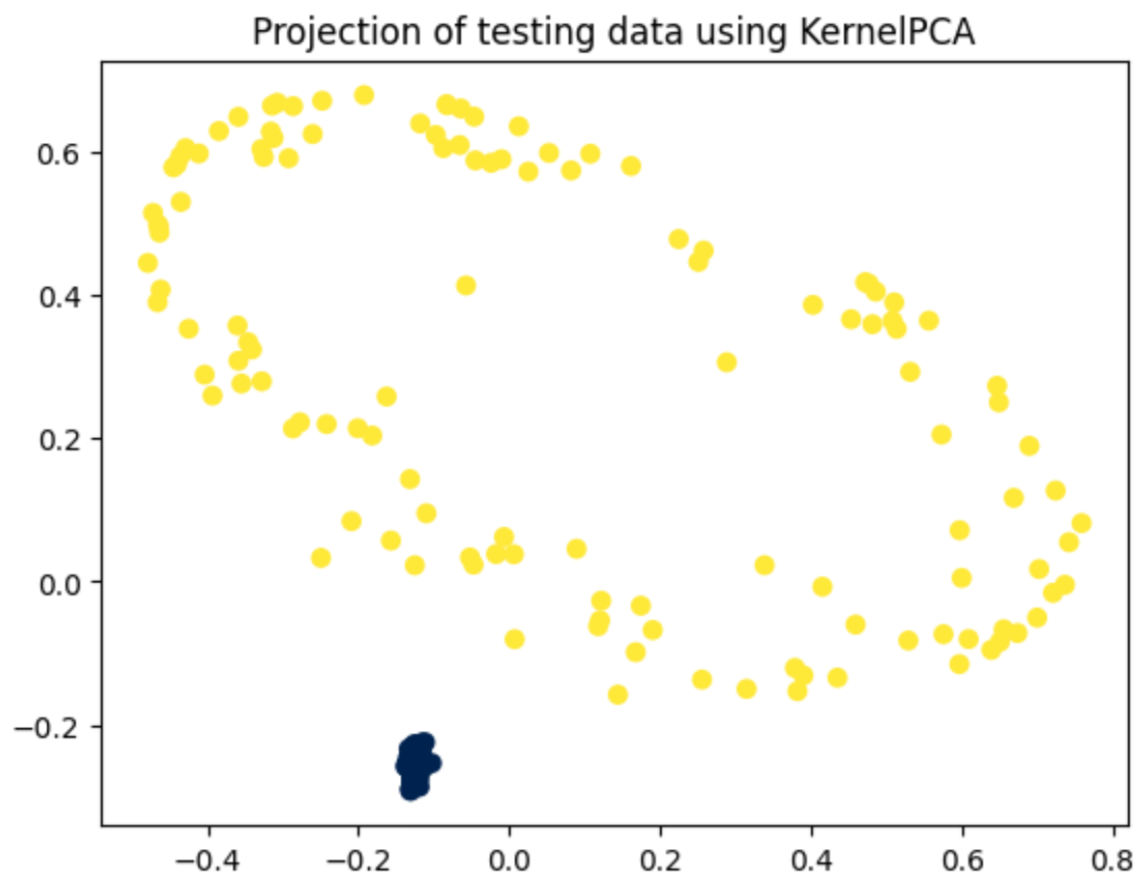
\includegraphics[width=0.4\textwidth]{figures/theory-example-figures/circles-kernelpca.png} }}
    \caption{both nonlinear methods on circles}
    \label{fig:nonlinear-methods-circles}
\end{figure}

In Figure \ref{fig:circles-kernelpca}, \gls{kpca} has also separated the data points from the circles. \gls{kpca} does an excellent job of maximizing the variance for the inner circle and separating the data points from each other. As can be seen, \gls{kpca} needs at least two dimensions to better differentiate between the two classes, unlike ISOMAP, which only needs one dimension.


Until now, we have presented some simple examples of the methods. More often than not, the number of reduced dimensions will not be two, as there will be much more relevant information in the other dimensions.